L'algorithme d'Angluin\cite{Angluin87} est un algorithme d'apprentissage actif d'automate. Il prend la forme d'un couple professeur/élève où l'élève applique l'algorithme d'Angluin $L^*$ en temps que tel pour apprendre l'automate et le professeur qui a accès au langage que l'élève veut apprendre.

\begin{figure}[H]
	\centering
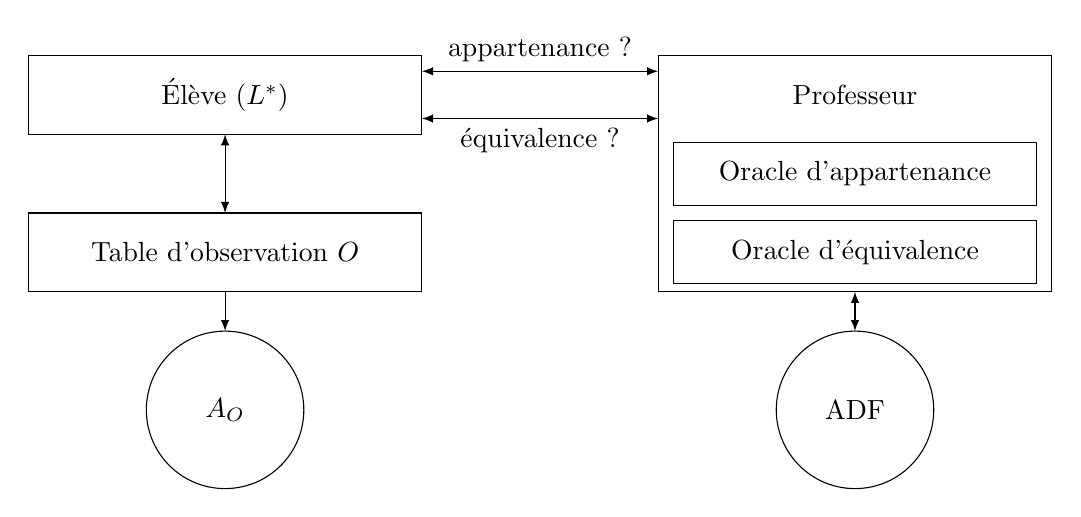
\begin{tikzpicture}
	\tikzset{>=latex}

	\draw (0,1) rectangle (5,0) node[pos=.5] {Élève ($L^*$)};
	\draw (8,1) rectangle (13,-2);

	\draw (8.2,-0.1) rectangle (12.8,-0.9) node[pos=.5] {Oracle d'appartenance};
	\draw (8.2,-1.1) rectangle (12.8,-1.9) node[pos=.5] {Oracle d'équivalence};

	\draw (0,-1) rectangle (5, -2) node[pos=.5] {Table d'observation $O$};

	\draw (10.5, -3.5) circle (1);
	\draw (2.5, -3.5) circle (1);

	\node[draw=none] at (10.5, 0.5) {Professeur} ;
	\node[draw=none] at (10.5,-3.5) {ADF};
	\node[draw=none] at (2.5,-3.5) {$A_O$};

	\draw[<->] (5,0.8) -- (8,0.8) node[pos=0.5,above] {appartenance ?};
	\draw[<->] (5,0.2) -- (8,0.2) node[pos=0.5,below] {équivalence ?};

	\draw[->] (2.5,-2) -- (2.5,-2.5);
	\draw[<->] (10.5, -2) -- (10.5,-2.5);
	\draw[<->] (2.5, 0) -- (2.5,-1);

\end{tikzpicture}
\caption{Vue schématique de l'algorithme d'Angluin}
\end{figure}

L'algorithme d'Angluin est nommé $L^*$ et est exécuté par l'élève. Par abus de language, il peut aussi désigner l'environnement complet dont il a besoin pour être fonctionnel.

Celui-ci consiste, côté élève, d'une table d'observation définie à la section \ref{ss:to}, et d'un automate $A_O$ construit à partir de cette table.

Côté professeur, il faut un langage régulier $L$ à apprendre, souvent représenté par un ADF. De plus, ce professeur contient deux oracles :
\begin{itemize}
	\item L'oracle d'appartenance. Soit un mot $w$. Appartient-il à $L$ ?
	\item L'oracle d'équivalence. Soit un automate $A_O$. Représente-t-il $L$ ? Si non, fournir un contre-exemple $w$.
\end{itemize}

\begin{theorem}
	S'appuyant sur un professeur pour un langage régulier $L\subseteq\Sigma^*$, un élève peut utiliser l'algorithme d'Angluin $L^*$ pour apprendre l'ADF canonique $A$ représentant $L$ en un temps polynimial à $n$ le nombre d'états de $A$ et $m$ le nombre de contre-exemples reçus du professeur.
	Il effectue $\mathcal{O}(n)$ requêtes d'équivalence et $\mathcal{O}(mn^2)$ requêtes d'appartenance.\cite{Angluin87}
\end{theorem}

\begin{corollary}
	Si les requêtes d'appartenance et d'équivalence se font en temps polynomial en la taille de $A$, $L^*$ est en temps polynomial.
\end{corollary}

Attention cependant : cet algorithme part du postulat que le langage étudié est régulier.

Les prochaines section introduisent les différentes notion notemment necéssaires à la compréhension du fonctionnement de la table d'observation.


% ██████  ██     ██
% ██   ██ ██     ██
% ██████  ██  █  ██
% ██   ██ ██ ███ ██
% ██   ██  ███ ███


\subsection{La relation \rw}

Soit un langage $L$ sur un alphabet $\Sigma$.

Soit la relation $R_L\subseteq\Sigma^*\times\Sigma^*$. Deux mots $x$ et $y$ respectent la \emph{relation de Myhill-Nérode $R_L$} si

$$\forall z \in \Sigma^*, xz \in L \Leftrightarrow yz \in L$$

Intuitivement, deux mots sont en relation si pour tout mot qu'on leur concatène, les deux mots résultants sont tous deux dans le langage $L$ ou non.

\begin{lemma}
	Cette relation est une relation d'équivalence. De plus, elle est congruente à droite. C'est à dire que si $xR_Ly$, alors pour tout symbole $a \in \Sigma$, $xaR_Lya$
\end{lemma}

\begin{proof}[Equivalence et Congruence à droite]
	Dire d'une relation qu'elle décrit une équivalence, revient à dire qu'elle est réflexive, transitive et symétrique
\begin{itemize}
		\item\textbf{Réflexive :} Soit $x \in \Sigma^*$. Soit $z \in \Sigma^*$. Montrer que $xR_Lx$ est vrai revient à montrer que $ xz \in L \Leftrightarrow xz \in L$ est vrai. $R_L$ est donc réflexive.
		\item \textbf{Symétrique :} Soient $x, y \in \Sigma^*$ tels que $xR_Ly$. Soit $w \in \Sigma^*$. Montrer que $yR_Lx$ revient à montrer que $ yw \in L \Leftrightarrow xw \in L$. Or, par hypothèse, $ xz \in L \Leftrightarrow yz \in L$, qui peut s'écrire aussi $ yz \in L \Leftrightarrow xz \in L$ pour tout $z \in \Sigma^*$, et en particulier $z=w$.
		\item \textbf{Transitive :} Soient $x,y,u \in \Sigma^*$ tels que $xR_Ly$ et $yR_Lz$. Soit $w \in \Sigma^*$. Comme $ xz \in L \Leftrightarrow yz \in L$ et $ yz \in L \Leftrightarrow uz \in L$ pour tout $z \in \Sigma^*$ (par hypothèse), c'est vrai en particulier pour $z=w$. Dès lors,  $ xw \in L \Leftrightarrow yw \in L$ et $ yw \in L \Leftrightarrow uw \in L$. Par transitivité de l'implication, on obtient $ xw \in L \Leftrightarrow uw \in L$, à savoir $xR_Lu$.
	\end{itemize}

	$R_L$ est congruente à droite. Soient $x,y \in \Sigma^*$ tels que $xR_Ly$. Soit $a \in \Sigma$. Par hypothèse, $ xz \in L \Leftrightarrow yz \in L$ pour tout $z \in \Sigma^*$. Cela doit donc être vrai en particulier pour le mot $z=aw$ avec $w$ quelconque. En remplaçant dans l'hypothèse, on obtient  $ xaw \in L \Leftrightarrow yaw \in L$. Ce qui montre que $xaR_Lya$.

\hfill$\square$
\end{proof}

% ███    ██ ███████ ██████   ██████  ██████  ███████
% ████   ██ ██      ██   ██ ██    ██ ██   ██ ██
% ██ ██  ██ █████   ██████  ██    ██ ██   ██ █████
% ██  ██ ██ ██      ██   ██ ██    ██ ██   ██ ██
% ██   ████ ███████ ██   ██  ██████  ██████  ███████

\subsection{Théorème de Myhill-Nerode}

	Avant d'introduire la théorème de Myhill-Nérode, il faut s'intéresser à la relation d'équivalence \rc, qui facilite l'écriture de la preuve du théorème.

	\begin{definition}[Relation \rc]
		Soit un automate \automaton. Soient deux mots $x,y\in\Sigma^*$. Alors la relation $xR_Cy$ est vraie si et seulement si $\hdelta(q_0,x)=\hdelta(q_0,y)$.
	\end{definition}

	Intuitivement, deux mots sont en relation \rc par rapport à un automate s'ils mènent à un même état dans celui-ci (ou des états équivalents).

	\begin{lemma}
		\rc est une relation d'équivalence congruente à droite.
	\end{lemma}

	\begin{proof}
		Prouver qu'une relation est dite d'équivalence, il faut prouver que celle-ci est transitive, réflexive et symétrique.
		Soit un automate \automaton.
		\begin{itemize}
		\item \rc est transitive. Soient $x,y,z\in\Sigma^*$. Supposons que $xR_Cy$ et $yR_Bz$. On a bien $\hdelta(q_0,x)=\hdelta(q_0,y)=\hdelta(q_0,z)$ par la transitivité de l'équivalence entre deux états.
		\item \rc est réflexive. Soit $y\in\Sigma^*$. On a bien $\hdelta(q_0,y)=\hdelta(q_0,y)$ par réflexiviré de l'équivalence sur un état.
		\item \rc est symétrique. Soient $x,y\in\Sigma^*$. Supposons que $xR_Cy$. On a bien $\hdelta(q_0,y)=\hdelta(q_0,x)$ par symétrie de l'équivalence entre deux états.
		\end{itemize}

		\rc est congruente à droite. Soient $x,y\in\Sigma^*$ tels que $xR_Cy$. Soit $z\in\Sigma^*$. Montrons que $xzR_Cyz$. $\hdelta(q_0,xz)=\hdelta(\hdelta(q_0,x),z)=\hdelta(\hdelta(q_0,y),z)=\hdelta(q_0,yz)$.

		\hfill$\square$
	\end{proof}

	\begin{theorem}
		Les trois énoncés suivants sont équivalents :
		\begin{enumerate}
			\item Un langage $L\subseteq\Sigma^*$ est accepté par un DFA.
			\item Il existe une congruence à droite sur $\Sigma^*$ d'index fini telle que $L$ est l'union de certaines classes d'équivalence.
			\item La relation d'équivalence $R_L$ est d'index fini.
		\end{enumerate}
	\end{theorem}


	\begin{proof}\label{proof:mn}
		La preuve d'équivalence se fait en prouvant chaque implication de façon cyclique :\\

		$(1)\rightarrow(2)$ Supposons que (1) soit vrai, c'est-à-dire que le langage $L$ est accepté par un automate déterministe \automaton. Considérons la relation d'équivalence congruente à droite \rc. Soit un mot $w\in\Sigma^*$. Alors tout mot $x\in\Sigma^*$ tel que $\hdelta(q_0,x)=\hdelta(q_0,w)$ appartient à la même classe d'équivalence $[w]$. Or, la fonction $\hdelta$ retourne un état $q\in Q$. Chaque classe d'équivalence sur $\Sigma$ correspond alors à un état de l'automate. Comme $Q$ est fini, \rc est d'index fini. De plus, un sous-ensemble des classes d'équivalences doit correspondre aux états acceptants $q\in F$. Alors, $L$ est l'union de ces classes d'équivalence.

		$(2)\rightarrow(3)$ Supposons qu'il existe une relation $E$ satisfaisant (2). Montrons que chaque classe de celle-ci est intégralement contenue dans une seule classe de \rw. Puisque $E$ est d'index fini, c'est un argument suffisant pour montrer que \rw est d'index fini. Soit $x,y$ tels que $xEy$. Comme $E$ est congruente à droite, pour tout mot $z \in \Sigma^*$, on sait que $xzEyz$. Comme $L$ est un union de ces classes d'équivalence, $xzEyz$ implique que $xz \in L \Leftrightarrow yz \in L$, ce qui revient à $xR_Wy$. Cela signifie que tout mot dans la classe d'équivalence de $x$ définie par $E$ se retrouve dans la même classe d'équivalence que $x$ cette fois définie par \rw. Ceci permet de conclure que chaque classe d'équivalence de $E$ est contenue dans une classe d'équivalence de \rw et donc que \rw est d'index fini.

		$(3)\rightarrow(1)$ Considérons la relation \rw définie précédemment. Soit un automate \automaton défini comme suit :
		\begin{itemize}
			\item Chaque état $q\in Q$ correspond à une classe d'équivalence de \rw.
			\item Comme \rw porte sur un langage, l'alphabet $\Sigma$ de celui-ci est déjà défini.
			\item Si $[[\epsilon]]$ est la classe d'équivalence de $\epsilon$ sur \rw, $q_0$ correspond à cette classe.
			\item Si $q$ représente $[[x]]$ et $q_1$ représente $[[xa]]$, alors $\delta(q,a)=q_1$. Cette définition est cohérente car \rw est congruente à droite.
			\item $F = \{[[x]]|x \in L\}$.
		\end{itemize}
		Cet automate est déterministe par la définition de $\delta$ et fini car $Q$ l'est, le nombre de classes de \rw étant fini par hypothèse. De plus, cet automate accepte tout mot $x\in L$ puisque $\delta(q_0,x)=[[x]]\in F$(par définition, puisque $x\in L$).
		\hfill$\square$
	\end{proof}


	\begin{corollary}
		La partie $(3)\rightarrow(1)$ de la preuve \ref{proof:mn} donne une méthode permettant de construire un ADF à partir des classes d'équivalences de la relation \rw.
	\end{corollary}

On peut prouver que l'automate obtenu de cette façon est l'automate minimal de $L$. Une preuve est disponible dans l'ouvrage \cite{Hopcroft79} en lien avec le théorème 3.10.


  % ████████  ██████
  %    ██    ██    ██
  %    ██    ██    ██
  %    ██    ██    ██
  %    ██     ██████

  \subsection{La table d'observation}\label{ss:to}

	Une \emph{table d'observation} est un tableau défini par $O=(R,S,T)$ avec $R\subseteq\Sigma^*$ un ensemble de mots \emph{représentants}, $S\subseteq\Sigma^*$ un ensmble de mots \emph{séparateurs} et $T:(R\bigcup R.\Sigma)\rightarrow\{0,1\}$ un mapping représentant le contenu de la table.\cite{Neider14}
	Soit un langage $L$ qui est en train d'être appris par l'algorithme d'Angluin. Soit un mot $w\in L$. Alors, $w$ appartient à une classe d'équivalence $[[u]]$ avec $u\in L$. Dans ce cas, $T(w)=1$. Au contraire, si $w\notin L$, alors $T(w)=0$.

	Pour une table d'observation $O$, deux mots $u,v$ peuvent être \emph{équivalents sur O}, c'est-à-dire $uR_Ov$. $u$ et $v$ sont équivalents sur $O$ si et seulement si $\forall w \in S, T(uw)=T(vw)$. Intuitivement, $uR_Ov$ si les lignes correspondant à leur classe d'équivalence ont la même séquence de $0$ et de $1$.

	\begin{proposition}
		Soient $u,v \in \Sigma^*$, un langage $L$ et une table d'observation $O$ associée à ce langage. Si $uR_Lv$, alors $uR_Ov$.
	\end{proposition}

	\begin{proof}
		Soient un langage $L$, $u,v \in \Sigma^*$ tels que $uR_Lv$ et une table d'observation $O$ associée à $L$.
		Comme $uR_Lv$, alors pour tout mot $w\in\Sigma^*$, $uw\in L \iff vw\in L$. C'est donc vrai en particulier pour tout $w\in S$. Dès lors, $\forall w \in S, T(uw)=T(vw)$.
		\hfill$\square$
	\end{proof}

	\begin{corollary}
		Le nombre de classes d'équivalence sur \ro est inférieur ou égal à celui de classes d'équivalence sur \rw.
	\end{corollary}

	Cette table $O$ représente la compréhension actuelle de l'élève du langage $L$. D'itération en itération, $R_O$ représente de mieux en mieux $R_L$ jusqu'à ce que l'automate induit de cette table soit jugé équivalent par le professeur.
	\todo{mentionner comment est construit l'automate en question ?}



	% ███████ ███████ ██████   ██████  ██████  ██   ██
	% ██      ██      ██   ██ ██      ██    ██ ██   ██
	% █████   █████   ██████  ██      ██    ██ ███████
	% ██      ██      ██   ██ ██      ██    ██ ██   ██
	% ██      ███████ ██   ██  ██████  ██████  ██   ██


\subsection{Fermeture et cohérence}

\subsubsection*{Fermeture}
La propriété de \emph{fermeture} s'exprime mathématiquement par

$$ \forall u \in R, \forall a \in \Sigma, \exists v \in R, ua R_O v$$

Cette propriété peut être vérifiée par cet algorithme, expliqué de façon visuelle sur la table O :

\begin{algorithm}[H]
	\begin{algorithmic}[1]
		\ENSURE si la fermeture est respectée ou non

		\FORALL {élément $w$ de la section $R$}
		\FORALL {symbole $a$ dans $\Sigma$}
			\IF {$wa$ est dans $R$}
				\STATE continuer
			\ELSE
				\STATE \COMMENT{$wa$ est dans $R.\Sigma$ par construction}
				\IF {La ligne de $wa$ dans $T$ est différente de celle de $w$}
					\RETURN Faux
				\ENDIF
			\ENDIF
		\ENDFOR
		\ENDFOR
		\RETURN Vrai
	\end{algorithmic}
	\caption{Vérification de la fermeture}\label{alg:fermeture}
\end{algorithm}

\subsubsection*{Cohérence}

La propriété de \emph{cohérence} se définit mathématiquement comme

$$ \forall u,v \in R, u R_O v \Rightarrow \forall a \in \Sigma, ua R_O va$$

Concrètement, il s'agit de prendre deux mots ($u,v$) dans $R$ ayant la même ligne dans $T$ et vérifier, pour chaque symbole ($a$), s'ils ($ua,va$) ont la même ligne dans $T$.

\begin{example}
	Soit la table d'observation O de la table \ref{tab:Oex} :

	\begin{table}[H]
		\centering
	\begin{tabular}{|c|c|c|}
		\hline
		$O$ & $\epsilon$ & a\\
		\hline
		$\epsilon$ & 0 & 0\\
		$a$ & 0 & 0\\
		\hline
		$aa$ & 0 & 1\\
		\hline
	\end{tabular}\caption{Table d'observation O}\label{tab:Oex}
\end{table}
	\vspace{0.5cm}
	Cette table n'est pas cohérente. En effet, $\epsilon R_O a$ mais en ajoutant le symbole $a\in \Sigma$, on obtient $\neg (a R_O aa)$. Les lignes ont les mêmes valeurs, mais les lignes obtenues par la concaténation du symbole $a$ ont des valeurs différentes.
\end{example}


%  █████  ██       ██████   ██████
% ██   ██ ██      ██       ██    ██
% ███████ ██      ██   ███ ██    ██
% ██   ██ ██      ██    ██ ██    ██
% ██   ██ ███████  ██████   ██████

\subsection{L'algorithme}\label{ss:a_exemple}

Le pseudocode de l'algorithme d'Angluin est fourni par l'algorithme \ref{alg:angluin}\cite{Neider14}. Celui-ci repose sur les oracles du professeur et l'algorithme \ref{alg:corr}, remplissant les lignes de $T$ encore vides. Le code est suivi d'un exemple d'exécution.

\begin{algo}[Algorithme d'Angluin $L^*$]\label{alg:angluin}
  \begin{algorithmic}[1]
    \REQUIRE Un professeur pour le langage régulier $L\subseteq\Sigma^*$
		\ENSURE Un automate canonique décrivant $L$
		\STATE Initialiser la table d'observation $O=(R,S,T)$ avec $R=S={\epsilon}$
		\STATE $corriger(O)$
		\REPEAT
			\WHILE {$O$ n'est pas fermée ou pas cohérente}
				\IF {$O$ n'est pas fermée}
					\STATE Choisir $r\in R$ et $a\in\Sigma$ tels que $[[ua]]_O\bigcap R=\emptyset$
					\STATE $R\leftarrow R\bigcup {ua}$
					\STATE $corriger(O)$
				\ENDIF
				\IF {$O$ n'est pas cohérente}
					\STATE Choisir $uR_Lv \in R, a\in\Sigma$ et $w\in S$ tels que $T(uaw)\neq T(vaw)$
					\STATE $S\leftarrow S \bigcup {aw}$
					\STATE $corriger(O)$
				\ENDIF
			\ENDWHILE
			\STATE Construire $A_O$
			\STATE Soumettre $A_O$ à l'oracle d'équivalence
			\IF {le professeur retourne un contre-exemple $u$}
				\STATE $R\leftarrow R\bigcup Pref(u)$
				\STATE $corriger(O)$
			\ENDIF
		\UNTIL {ce que le professeur réponde "oui" à l'équivalence}
		\RETURN $A_O$
  \end{algorithmic}
\end{algo}

\begin{algo}[$corriger(O)$]\label{alg:corr}
  \begin{algorithmic}[1]
		\REQUIRE une table d'observation $O$, un professeur pour le langage régulier $L\subseteq\Sigma^*$
		\ENSURE les entrées de $O$ sont valide dans $L$
		\FORALL {entrée $u \in (R\bigcup R\Sigma)$ pour laquelle $T(u)$ n'est pas encore définie}
			\IF {$u\in L$ par le test d'appartenance }
				\STATE $T(u)\leftarrow 1$
			\ELSE
				\STATE $T(u)\leftarrow 0$
			\ENDIF
		\ENDFOR
	\end{algorithmic}
\end{algo}

Considérons l'automate $A_3$ de la figure \ref{fig:a3} construit à la section \ref{ss:mini} sur la minimisation.

%\todo{Marquer la différence entre $R_L$ et $R_O$}

\subsubsection{Première itération}

L'algorithme d'Angluin précise, pour son cas de base, une initialisation de la table $T$ avec les ensembles $R$ et $S$ contenant uniquement $\epsilon$. Le champ $R.\{a,b\}$ ($R.\Sigma$) est rempli via des requêtes d'appartenance sur les mots $a$ et $b$.

\begin{minipage}{0.5\linewidth}
	\centering
	\begin{tabular}{|c|c|}
		\hline
		$O_0$ & $\epsilon$\\
		\hline
		$\epsilon$ & 0\\
		\hline
		$a$ & 0\\
		$b$ & 0\\
		\hline
	\end{tabular}
\end{minipage}
\begin{minipage}{0.5\linewidth}
	\centering
	\begin{figure}[H]
		\centering
		\begin{tikzpicture}[->,>=stealth',shorten >=1pt,auto,node distance=3cm, semithick, bend angle=10]
		\tikzstyle{every state}=[circle]
		\node[initial, state] (A) {$[[\epsilon]]$};
		\path (A) edge [loop above] node {a,b} (A);
		\end{tikzpicture}
		\caption*{Automate $O_0$}
	\end{figure}
\end{minipage}


\vspace{1cm}
L'étape suivante consiste à vérifier la fermeture de la table d'observation $O_0$. Pour rappel :

$$ \forall u \in R, \forall a \in \Sigma, \exists v \in R, ua R_O v$$

Intuitivement, pour chaque symbole (ici, $\{a,b\}$, et ce sera vrai jusqu'à la dernière itération), tout mot candidat (dans $R$, la partie supérieure de la table) doit se retrouver, complété de ce symbole, dans une classe d'équivalence d'un autre candidat de $R$. Ici, de toute évidence, les mots $a$ et $b$ sont dans la même classe d'équivalence que $\epsilon$. Dès lors, la propriété de fermeture est respectée.

Si la fermeture est respectée, alors la question de la cohérence se pose. Pour rappel :

$$ \forall u,v \in R, u R_O v \Rightarrow \forall a \in \Sigma, ua R_O va$$

Intuitivement, si deux candidats semblent être dans la même classe d'équivalence (leur lignes dans la table supérieure sont identiques), alors pour n'importe quel symbole, les deux nouveaux mots sont également dans une même classe d'équivalence (leur lignes, potentiellement dans la partie inférieure de la table, sont identiques). N'ayant qu'un seul candidat, cette propriété est forcément respectée ($R_L$ est réflexive).

Les deux propriétés étant respectées, les classes d'équivalences sont calculées (trivialement ici), et un automate $O_0$ est proposé à l'enseignant pour vérification.

Sur cette itération, un automate initial a été proposé, et aucun état final ne pouvant être atteint avec un seul symbole, la version est minime.

\subsubsection{Seconde itération}

L'enseignant répond que non, les automates ne sont pas équivalents. Il fourni le contre-exemple $ba$. Comme il est rejeté par $O_0$, cela signifie qu'il est accepté par $A_3$. Une nouvelle table est alors construite, en ajoutant $ba$ et ses préfixes (ici, juste $b$) à $R$. $R.\Sigma$ est calculé et les mots n'ayant pas encore reçu une valeur dans $T$ sont soumis à l'enseignant pour un test d'appartenance.
Les valeurs ajoutées ou modifiées dans la table d'observation sont mises en évidence \textcolor{red}{en rouge}.
\vspace{1cm}

\begin{minipage}{0.25\linewidth}
	\centering
	\begin{tabular}{|c|c|}
		\hline
		$O_1$ & $\epsilon$\\
		\hline
		$\epsilon$ & 0\\
		\textcolor{red}{$b$} & \textcolor{red}{0}\\
		\textcolor{red}{$ba$} & \textcolor{red}{1}\\
		\hline
		$a$ & 0\\
		\textcolor{red}{$bb$} & \textcolor{red}{0}\\
		\textcolor{red}{$baa$} & \textcolor{red}{1}\\
		\textcolor{red}{$bab$} & \textcolor{red}{1}\\
		\hline
	\end{tabular}
\end{minipage}
\begin{minipage}{0.25\linewidth}
	\centering
	\begin{tabular}{|c|cc|}
		\hline
		$O_2$ & $\epsilon$ & \textcolor{red}{$a$}\\
		\hline
		$\epsilon$ & 0& \textcolor{red}{0}\\
		$b$ & 0&\textcolor{red}{1}\\
		$ba$ & 1&\textcolor{red}{1}\\
		\hline
		$a$ & 0&\textcolor{red}{0}\\
		$bb$ & 0&\textcolor{red}{1}\\
		$baa$ & 1&\textcolor{red}{1}\\
		$bab$ & 1&\textcolor{red}{1}\\
		\hline
	\end{tabular}
\end{minipage}
\begin{minipage}{0.5\linewidth}
	\centering
	\begin{figure}[H]
		\centering
		\begin{tikzpicture}[->,>=stealth',shorten >=1pt,auto,node distance=3cm, semithick, bend angle=10]
		\tikzstyle{every state}=[circle]

		\node[initial, state] (A) {$[[\epsilon]]$};
		\node[state] (B) [right of=A] {$[[b]]$};
		\node[accepting, state] [right of=B] (C) {$[[ba]]$};

		\path
		(A) edge [loop above] node {a} (A)
		(A) edge node {b} (B)
		(B) edge node {a} (C)
		(B) edge [loop above] node {b} (B)
		(C) edge [loop above] node {a,b} (C);


		\end{tikzpicture}
		\caption*{Automate $O_2$}
	\end{figure}
\end{minipage}

\vspace{1cm}
Comme pour la première itération, la fermeture est testée, suivie de la cohérence. Celle-ci n'est pas respectée : si on considère les mots $\epsilon$ et $b$, qui ont la même ligne dans la table $T$ ($\epsilon R_O b$), le symbole $a$, on obtient les mots $a$ et $ba$ qui n'ont pas la même ligne : ($\neg a R_O ba$). Le symbole $a$ est alors ajouté à $S$ et une nouvelle table $O_2$ est calculée.

La fermeture étant déjà vérifiée, la question de la cohérence est reposée, et cette fois-ci elle est vérifiée ; l'automate est construit et proposé à l'enseignant.

Sur cette itération, l'algorithme a reçu le mot $ba$ comme étant accepté. Il a du ajouter $a$ à $S$ pour permettre de différencier certains états. L'automate se voit ajouter les états $[[b]]$ et $[[ba]]$.

\subsubsection{Troisième itération}

Suivant toujours l'algorithme de comparaison d'automates détaillé dans la section \ref{ss:eqauto}, l'enseignant découvre qu'ils sont différents.

Il sort le contre-exemple $aaba$. Si c'est un contre-exemple et qu'il est accepté par $O_2$, c'est qu'il ne l'est pas (0) par $A_4$. Une nouvelle table $O_3$ doit être construite.

\begin{minipage}{0.25\linewidth}
	\centering
	\begin{tabular}{|c|cc|}
		\hline
		$O_3$ & $\epsilon$ & $a$\\
		\hline
		$\epsilon$ & 0 &0\\
		\textcolor{red}{$a$}&\textcolor{red}{0}&\textcolor{red}{0}\\
		$b$&0&1\\
		\textcolor{red}{$aa$}&\textcolor{red}{0}&\textcolor{red}{0}\\
		$ba$&1&1\\
		\textcolor{red}{$aab$}&\textcolor{red}{0}&\textcolor{red}{0}\\
		\textcolor{red}{$aaba$}&\textcolor{red}{0}&\textcolor{red}{0}\\
		\hline
		\textcolor{red}{$ab$}&\textcolor{red}{0}&\textcolor{red}{1}\\
		$bb$&0&1\\
		\textcolor{red}{$aaa$}&\textcolor{red}{0}&\textcolor{red}{0}\\
		$baa$&1&1\\
		$bab$&1&1\\
		\textcolor{red}{$aabb$}&\textcolor{red}{0}&\textcolor{red}{0}\\
		\textcolor{red}{$aabaa$}&\textcolor{red}{0}&\textcolor{red}{0}\\
		\textcolor{red}{$aabab$}&\textcolor{red}{0}&\textcolor{red}{0}\\
		\hline
	\end{tabular}
\end{minipage}
\begin{minipage}{0.33\linewidth}
	\centering
	\begin{tabular}{|c|cc|}
		\hline
		$O_4$ & $\epsilon$ & $a$\\
		\hline
		$\epsilon$ & 0 &0\\
		$a$&0&0\\
		$b$&0&1\\
		$aa$&0&0\\
		\textcolor{red}{$ab$}&\textcolor{red}{0}&\textcolor{red}{1}\\
		$ba$&1&1\\
		$aab$&0&0\\
		$aaba$&0&0\\
		\hline
		$bb$&0&1\\
		$aaa$&0&0\\
		\textcolor{red}{$aba$}&\textcolor{red}{1}&\textcolor{red}{1}\\
		\textcolor{red}{$abb$}&\textcolor{red}{0}&\textcolor{red}{1}\\
		$baa$&1&1\\
		$bab$&1&1\\
		$aabb$&0&0\\
		$aabaa$&0&0\\
		$aabab$&0&0\\
		\hline
	\end{tabular}
\end{minipage}
\begin{minipage}{0.33\linewidth}
	\centering
	\begin{tabular}{|c|ccccc|}
		\hline
		$O_7$ & $\epsilon$ & $a$&\textcolor{red}{$b$}&\textcolor{red}{$ab$}&\textcolor{red}{$ba$}\\
		\hline
		$\epsilon$&0&0&\textcolor{red}{0}&\textcolor{red}{1}&\textcolor{red}{1}\\
		$a$&0&0&\textcolor{red}{0}&\textcolor{red}{0}&\textcolor{red}{1}\\
		$b$&0&1&\textcolor{red}{0}&\textcolor{red}{1}&\textcolor{red}{1}\\
		$aa$&0&0&\textcolor{red}{0}&\textcolor{red}{0}&\textcolor{red}{0}\\
		$ab$&0&1&\textcolor{red}{0}&\textcolor{red}{1}&\textcolor{red}{1}\\
		$ba$&1&1&\textcolor{red}{1}&\textcolor{red}{1}&\textcolor{red}{1}\\
		$aab$&0&0&\textcolor{red}{0}&\textcolor{red}{0}&\textcolor{red}{0}\\
		$aaba$&0&0&\textcolor{red}{0}&\textcolor{red}{0}&\textcolor{red}{0}\\
		\hline
		$bb$&0&1&\textcolor{red}{0}&\textcolor{red}{1}&\textcolor{red}{1}\\
		$aaa$&0&0&\textcolor{red}{0}&\textcolor{red}{0}&\textcolor{red}{0}\\
		$aba$&1&1&\textcolor{red}{1}&\textcolor{red}{1}&\textcolor{red}{1}\\
		$abb$&0&1&\textcolor{red}{0}&\textcolor{red}{1}&\textcolor{red}{1}\\
		$baa$&1&1&\textcolor{red}{1}&\textcolor{red}{1}&\textcolor{red}{1}\\
		$bab$&1&1&\textcolor{red}{1}&\textcolor{red}{1}&\textcolor{red}{1}\\
		$aabb$&0&0&\textcolor{red}{0}&\textcolor{red}{0}&\textcolor{red}{0}\\
		$aabaa$&0&0&\textcolor{red}{0}&\textcolor{red}{0}&\textcolor{red}{0}\\
		$aabab$&0&0&\textcolor{red}{0}&\textcolor{red}{0}&\textcolor{red}{0}\\
		\hline
	\end{tabular}
\end{minipage}

	\begin{figure}[H]
		\centering
		\begin{tikzpicture}[->,>=stealth',shorten >=1pt,auto,node distance=3cm, semithick, bend angle=10]
		\tikzstyle{every state}=[circle]

		\node[initial, state] (A) {$[[\epsilon]]$};
		\node[state] (B) [above right of=A] {$[[a]]$};
		\node [state] (E) [right of=B] {$[[aa]]$};
		\node[state] (C) [below right of =A] {$[[b]]$};
		\node[accepting, state] [right of=C] (D) {$[[ba]]$};

		\path
		(A) edge node {a} (B)
		(A) edge node {b} (C)
		(B) edge node {b} (C)
		(B) edge node {a} (E)
		(C) edge [loop below] node {b} (C)
		(C) edge node {a} (D)
		(D) edge [loop above] node {a,b} (D)
		(E) edge [loop below] node {a,b} (E);

		\end{tikzpicture}
		\caption*{Automate $O_7$}
	\end{figure}


Ayant reçu $aaba$, ce mot et tous ses préfixes sont ajoutés à la table. L'extension $R.\Sigma$ est recalculée et la table $O_3$ est construite.

Un manquement à la fermeture est détecté : le mot $a$. En effet, en lui ajoutant le symbole $b$, on obtient $ab$ qui n'est ni dans $R$ ni en relation $R_O$ avec $a$. $ab$ est alors ajouté à $R$, et $R.\Sigma$ est étendu. La nouvelle table, $O_4$ est de nouveau testée.

$O_4$ ne respecte pas la cohérence. Les mots $\epsilon$ et $aa$ respectent \ro (leur ligne a la même valeur dans la table) mais $\neg b R_O aab$. $b$ est alors ajouté à $S$ et une nouvelle colonne associée est ajoutée à la table, donnant le table $O_5$. Celle-ci a toujours un soucis de cohérence entre $\epsilon$ et $aa$, menant à l'ajout de $ab$ à $S$ et à la création de $O_6$. Finalement, pour régler le soucis de cohérence dans $O_6$ entre $a$ et $aa$, le mot $ba$ est ajouté à $S$ et une table $O_7$ est ainsi créée avec la nouvelle colonne associée.

Cette table $O_7$ respectant la fermeture et la cohérence, l'automate associé $O_7$ est construit et soumis à l'enseignant pour être comparé à $A_3$. Celui-ci valide l'égalité et l'algorithme s'arrête : l'automate a été construit.
